% Options for packages loaded elsewhere
\PassOptionsToPackage{unicode}{hyperref}
\PassOptionsToPackage{hyphens}{url}
%
\documentclass[
]{article}
\usepackage{amsmath,amssymb}
\usepackage{lmodern}
\usepackage{ifxetex,ifluatex}
\ifnum 0\ifxetex 1\fi\ifluatex 1\fi=0 % if pdftex
  \usepackage[T1]{fontenc}
  \usepackage[utf8]{inputenc}
  \usepackage{textcomp} % provide euro and other symbols
\else % if luatex or xetex
  \usepackage{unicode-math}
  \defaultfontfeatures{Scale=MatchLowercase}
  \defaultfontfeatures[\rmfamily]{Ligatures=TeX,Scale=1}
\fi
% Use upquote if available, for straight quotes in verbatim environments
\IfFileExists{upquote.sty}{\usepackage{upquote}}{}
\IfFileExists{microtype.sty}{% use microtype if available
  \usepackage[]{microtype}
  \UseMicrotypeSet[protrusion]{basicmath} % disable protrusion for tt fonts
}{}
\makeatletter
\@ifundefined{KOMAClassName}{% if non-KOMA class
  \IfFileExists{parskip.sty}{%
    \usepackage{parskip}
  }{% else
    \setlength{\parindent}{0pt}
    \setlength{\parskip}{6pt plus 2pt minus 1pt}}
}{% if KOMA class
  \KOMAoptions{parskip=half}}
\makeatother
\usepackage{xcolor}
\IfFileExists{xurl.sty}{\usepackage{xurl}}{} % add URL line breaks if available
\IfFileExists{bookmark.sty}{\usepackage{bookmark}}{\usepackage{hyperref}}
\hypersetup{
  pdftitle={Raport\_Projet\_AcLab},
  pdfauthor={Dahiez Burdy},
  hidelinks,
  pdfcreator={LaTeX via pandoc}}
\urlstyle{same} % disable monospaced font for URLs
\usepackage[margin=1in]{geometry}
\usepackage{color}
\usepackage{fancyvrb}
\newcommand{\VerbBar}{|}
\newcommand{\VERB}{\Verb[commandchars=\\\{\}]}
\DefineVerbatimEnvironment{Highlighting}{Verbatim}{commandchars=\\\{\}}
% Add ',fontsize=\small' for more characters per line
\usepackage{framed}
\definecolor{shadecolor}{RGB}{248,248,248}
\newenvironment{Shaded}{\begin{snugshade}}{\end{snugshade}}
\newcommand{\AlertTok}[1]{\textcolor[rgb]{0.94,0.16,0.16}{#1}}
\newcommand{\AnnotationTok}[1]{\textcolor[rgb]{0.56,0.35,0.01}{\textbf{\textit{#1}}}}
\newcommand{\AttributeTok}[1]{\textcolor[rgb]{0.77,0.63,0.00}{#1}}
\newcommand{\BaseNTok}[1]{\textcolor[rgb]{0.00,0.00,0.81}{#1}}
\newcommand{\BuiltInTok}[1]{#1}
\newcommand{\CharTok}[1]{\textcolor[rgb]{0.31,0.60,0.02}{#1}}
\newcommand{\CommentTok}[1]{\textcolor[rgb]{0.56,0.35,0.01}{\textit{#1}}}
\newcommand{\CommentVarTok}[1]{\textcolor[rgb]{0.56,0.35,0.01}{\textbf{\textit{#1}}}}
\newcommand{\ConstantTok}[1]{\textcolor[rgb]{0.00,0.00,0.00}{#1}}
\newcommand{\ControlFlowTok}[1]{\textcolor[rgb]{0.13,0.29,0.53}{\textbf{#1}}}
\newcommand{\DataTypeTok}[1]{\textcolor[rgb]{0.13,0.29,0.53}{#1}}
\newcommand{\DecValTok}[1]{\textcolor[rgb]{0.00,0.00,0.81}{#1}}
\newcommand{\DocumentationTok}[1]{\textcolor[rgb]{0.56,0.35,0.01}{\textbf{\textit{#1}}}}
\newcommand{\ErrorTok}[1]{\textcolor[rgb]{0.64,0.00,0.00}{\textbf{#1}}}
\newcommand{\ExtensionTok}[1]{#1}
\newcommand{\FloatTok}[1]{\textcolor[rgb]{0.00,0.00,0.81}{#1}}
\newcommand{\FunctionTok}[1]{\textcolor[rgb]{0.00,0.00,0.00}{#1}}
\newcommand{\ImportTok}[1]{#1}
\newcommand{\InformationTok}[1]{\textcolor[rgb]{0.56,0.35,0.01}{\textbf{\textit{#1}}}}
\newcommand{\KeywordTok}[1]{\textcolor[rgb]{0.13,0.29,0.53}{\textbf{#1}}}
\newcommand{\NormalTok}[1]{#1}
\newcommand{\OperatorTok}[1]{\textcolor[rgb]{0.81,0.36,0.00}{\textbf{#1}}}
\newcommand{\OtherTok}[1]{\textcolor[rgb]{0.56,0.35,0.01}{#1}}
\newcommand{\PreprocessorTok}[1]{\textcolor[rgb]{0.56,0.35,0.01}{\textit{#1}}}
\newcommand{\RegionMarkerTok}[1]{#1}
\newcommand{\SpecialCharTok}[1]{\textcolor[rgb]{0.00,0.00,0.00}{#1}}
\newcommand{\SpecialStringTok}[1]{\textcolor[rgb]{0.31,0.60,0.02}{#1}}
\newcommand{\StringTok}[1]{\textcolor[rgb]{0.31,0.60,0.02}{#1}}
\newcommand{\VariableTok}[1]{\textcolor[rgb]{0.00,0.00,0.00}{#1}}
\newcommand{\VerbatimStringTok}[1]{\textcolor[rgb]{0.31,0.60,0.02}{#1}}
\newcommand{\WarningTok}[1]{\textcolor[rgb]{0.56,0.35,0.01}{\textbf{\textit{#1}}}}
\usepackage{graphicx}
\makeatletter
\def\maxwidth{\ifdim\Gin@nat@width>\linewidth\linewidth\else\Gin@nat@width\fi}
\def\maxheight{\ifdim\Gin@nat@height>\textheight\textheight\else\Gin@nat@height\fi}
\makeatother
% Scale images if necessary, so that they will not overflow the page
% margins by default, and it is still possible to overwrite the defaults
% using explicit options in \includegraphics[width, height, ...]{}
\setkeys{Gin}{width=\maxwidth,height=\maxheight,keepaspectratio}
% Set default figure placement to htbp
\makeatletter
\def\fps@figure{htbp}
\makeatother
\setlength{\emergencystretch}{3em} % prevent overfull lines
\providecommand{\tightlist}{%
  \setlength{\itemsep}{0pt}\setlength{\parskip}{0pt}}
\setcounter{secnumdepth}{-\maxdimen} % remove section numbering
\ifluatex
  \usepackage{selnolig}  % disable illegal ligatures
\fi

\title{Raport\_Projet\_AcLab}
\author{Dahiez Burdy}
\date{20/05/2021}

\begin{document}
\maketitle

\hypertarget{introduction}{%
\section{Introduction}\label{introduction}}

Sur ce tp, nous allons annalyser des données météo enregistré par une
sonde météorologique conçu par la filière IOT Maker, ces données sont
constitué, de la date et heure, l'humidité, pression, temperature,
intensité lumineuse et la pluie.avec ces données nous allons étudier
quelles sont les facteurs qui annoncent la pluie. comme par exemple si
le taux d'humidité augmente avant qu'il pleuve.

\begin{itemize}
\tightlist
\item
  Hypothèse :
\end{itemize}

Nous émetons l'hypothèse que la diminution de pression est un facteur
annonciateur de la pluie.

Nous émetons l'hypothèse que le facteur d'humidité est un facteur
annonciateur de la pluie plus conséquent selon la saison.

Nous émetons l'hypothèse que la température diminue avant l'arrivé de la
pluie.

Nous émetons l'hypothèse que si nous detectons la présence de la pluie
moins de 10 minutes avant la prédiction, la probabilitée qu'il pleuve
augmente.

Nous émétons l'hypothèse que la nuit est un facteur annonciateur de la
pluie.

Est il possible de creer un algorythme de prédiction d'apparition de la
pluie ayant une precision de plus de 0.8 ?

\hypertarget{analyse-de-la-pression}{%
\section{Analyse de la Pression}\label{analyse-de-la-pression}}

Pour etre sûr que cette hypothése est intéréssante nous allons recherché
la corrélation entre la Pression atmosphérique et l'apparition de pluie
.Nous voulons déja savoir si la temperature à une corrélation avec la
pressions athmosphérique . Pour ce faire nous executons ces commandes
suivantes :

\begin{Shaded}
\begin{Highlighting}[]
\FunctionTok{cor.test}\NormalTok{(data\_meteo}\SpecialCharTok{$}\NormalTok{pressure , data\_meteo}\SpecialCharTok{$}\NormalTok{temperature) }\CommentTok{\#{-}0.31}
\end{Highlighting}
\end{Shaded}

\begin{verbatim}
## 
##  Pearson's product-moment correlation
## 
## data:  data_meteo$pressure and data_meteo$temperature
## t = -90.622, df = 72255, p-value < 2.2e-16
## alternative hypothesis: true correlation is not equal to 0
## 95 percent confidence interval:
##  -0.3259972 -0.3129026
## sample estimates:
##        cor 
## -0.3194652
\end{verbatim}

la corrélation entre la température et la pression est de -0.31 avec un
p-value très faible , la temperarute à donc une influence sur la
pression . Sachant que le cycle du soleil joue un grand rôle sur la
température relevé nous décidons de ne traiter les données effectué
entre 7 heures et 19 heures .

\begin{Shaded}
\begin{Highlighting}[]
\NormalTok{data\_meteo\_season}\SpecialCharTok{$}\NormalTok{hour }\OtherTok{\textless{}{-}} \FunctionTok{strtoi}\NormalTok{(}\FunctionTok{str\_sub}\NormalTok{(data\_meteo\_season}\SpecialCharTok{$}\NormalTok{date..date, }\DecValTok{13}\NormalTok{, }\DecValTok{14}\NormalTok{))}

\NormalTok{data\_meteo\_jour}\OtherTok{\textless{}{-}} \FunctionTok{filter}\NormalTok{(data\_meteo\_season , hour }\SpecialCharTok{\textgreater{}=}  \DecValTok{7}\NormalTok{)}

\NormalTok{data\_meteo\_jour }\OtherTok{\textless{}{-}}  \FunctionTok{filter}\NormalTok{(data\_meteo\_jour , hour }\SpecialCharTok{\textless{}=}  \DecValTok{21}\NormalTok{)}
\end{Highlighting}
\end{Shaded}

On observe que de 8 a 10 heures les données ne sont pas traitées par
problème de selection dans R studio .

Maintenant on vas observer la correlation entre la pression et la pluie
pour une journée les de 7 heure à 21 heures

\begin{Shaded}
\begin{Highlighting}[]
\FunctionTok{cor.test}\NormalTok{(data\_meteo\_jour}\SpecialCharTok{$}\NormalTok{pressure , data\_meteo\_jour}\SpecialCharTok{$}\NormalTok{rain) }\CommentTok{\#{-}0.07924169 }
\end{Highlighting}
\end{Shaded}

\begin{verbatim}
## 
##  Pearson's product-moment correlation
## 
## data:  data_meteo_jour$pressure and data_meteo_jour$rain
## t = -15.425, df = 42047, p-value < 2.2e-16
## alternative hypothesis: true correlation is not equal to 0
## 95 percent confidence interval:
##  -0.08451056 -0.06550187
## sample estimates:
##         cor 
## -0.07501303
\end{verbatim}

On observe ici une très légére correlation négative , est un p-value
très faible . Nous en déduisons donc que l'analyse de l'évolution de la
préssion athmosphérique ne peut pas nous permettre de determiner
fiablement si la pluie risque de tomber dans l'heure .

Pour confirmer graphiquement que la Pression athmosphérique n'est pas un
bon indicateur nous avons extrait les données se trouvant juste avant
une période de pluie . Pour faire plus simple nous selectionnons les
données se trouvant entre chaque péridode de pluie grace un un code
python.

\begin{Shaded}
\begin{Highlighting}[]
\CommentTok{\#path\_to\_python \textless{}{-} "C:/Python39/python.exe"}
\CommentTok{\#use\_python(path\_to\_python, required = TRUE)}
\CommentTok{\# C:\textbackslash{}\textbackslash{}Users\textbackslash{}\textbackslash{}sburd\textbackslash{}\textbackslash{}OneDrive\textbackslash{}\textbackslash{}Bureau\textbackslash{}\textbackslash{}Semestre2\textbackslash{}\textbackslash{}Projet\_Data\textbackslash{}Stat\textbackslash{}\textbackslash{}Stat\_Projet\_Data\textbackslash{}\textbackslash{}RecupPluieTrue.py}
\FunctionTok{py\_install}\NormalTok{(}\StringTok{"pandas"}\NormalTok{)}

\FunctionTok{source\_python}\NormalTok{(}\StringTok{"C:}\SpecialCharTok{\textbackslash{}\textbackslash{}}\StringTok{Users}\SpecialCharTok{\textbackslash{}\textbackslash{}}\StringTok{sburd}\SpecialCharTok{\textbackslash{}\textbackslash{}}\StringTok{OneDrive}\SpecialCharTok{\textbackslash{}\textbackslash{}}\StringTok{Bureau}\SpecialCharTok{\textbackslash{}\textbackslash{}}\StringTok{Semestre2}\SpecialCharTok{\textbackslash{}\textbackslash{}}\StringTok{Projet\_Data}\SpecialCharTok{\textbackslash{}\textbackslash{}}\StringTok{Stat}\SpecialCharTok{\textbackslash{}\textbackslash{}}\StringTok{Stat\_Projet\_Data}\SpecialCharTok{\textbackslash{}\textbackslash{}}\StringTok{RecupPluieTrue.py"}\NormalTok{)}
\CommentTok{\#monCsv \textless{}{-} openMonCsv("C:\textbackslash{}\textbackslash{}Users\textbackslash{}\textbackslash{}sburd\textbackslash{}\textbackslash{}OneDrive\textbackslash{}\textbackslash{}Bureau\textbackslash{}\textbackslash{}Semestre2\textbackslash{}\textbackslash{}Projet\_Data\textbackslash{}\textbackslash{}DataV2\textbackslash{}\textbackslash{}dataTrainSortiPluie1.csv")}
\NormalTok{monCsv }\OtherTok{\textless{}{-}} \FunctionTok{openMonCsv}\NormalTok{(}\StringTok{"C:}\SpecialCharTok{\textbackslash{}\textbackslash{}}\StringTok{Users}\SpecialCharTok{\textbackslash{}\textbackslash{}}\StringTok{sburd}\SpecialCharTok{\textbackslash{}\textbackslash{}}\StringTok{OneDrive}\SpecialCharTok{\textbackslash{}\textbackslash{}}\StringTok{Bureau}\SpecialCharTok{\textbackslash{}\textbackslash{}}\StringTok{Semestre2}\SpecialCharTok{\textbackslash{}\textbackslash{}}\StringTok{Projet\_Data}\SpecialCharTok{\textbackslash{}\textbackslash{}}\StringTok{DataV2}\SpecialCharTok{\textbackslash{}\textbackslash{}}\StringTok{dataTrainSorti.csv"}\NormalTok{)}
\NormalTok{heureAdd }\OtherTok{\textless{}{-}} \FunctionTok{AddHour}\NormalTok{(monCsv)}
\NormalTok{maTabPluie }\OtherTok{\textless{}{-}} \FunctionTok{trie}\NormalTok{(heureAdd)}
\NormalTok{tabDataFrame }\OtherTok{\textless{}{-}} \FunctionTok{SubsetData}\NormalTok{(maTabPluie)}
\NormalTok{newCollection }\OtherTok{\textless{}{-}} \FunctionTok{TrieTaille}\NormalTok{(}\DecValTok{120}\NormalTok{,}\DecValTok{180}\NormalTok{,tabDataFrame , heureAdd)}
\end{Highlighting}
\end{Shaded}

La varable NewCollection est une liste de dataFrame de periode d'avant
pluie comprise entre 120 et 150 données ( correspondant aproximativement
à une journée de 24 heures ).

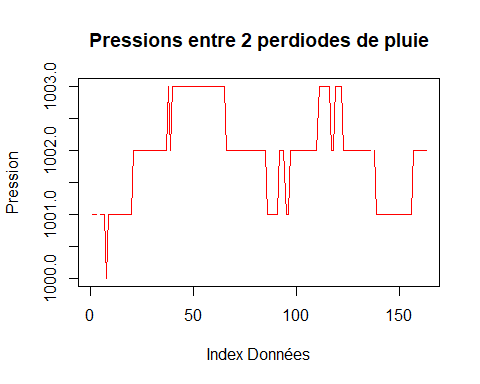
\includegraphics{Rapport_Projet_Data_files/figure-latex/pressure-1.pdf}
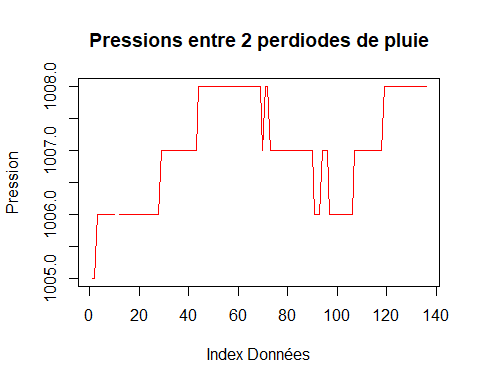
\includegraphics{Rapport_Projet_Data_files/figure-latex/pressure-2.pdf}
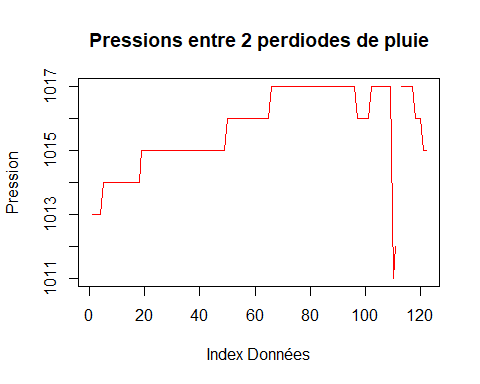
\includegraphics{Rapport_Projet_Data_files/figure-latex/pressure-3.pdf}
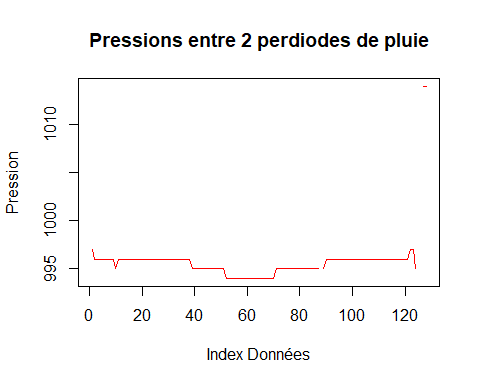
\includegraphics{Rapport_Projet_Data_files/figure-latex/pressure-4.pdf}
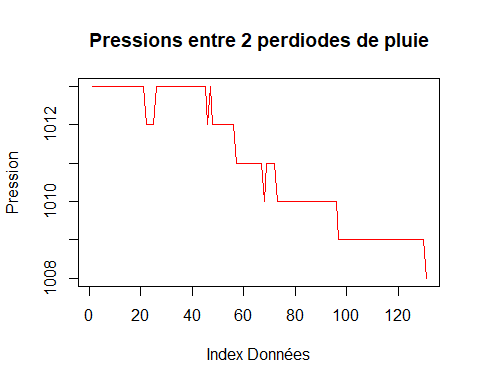
\includegraphics{Rapport_Projet_Data_files/figure-latex/pressure-5.pdf}
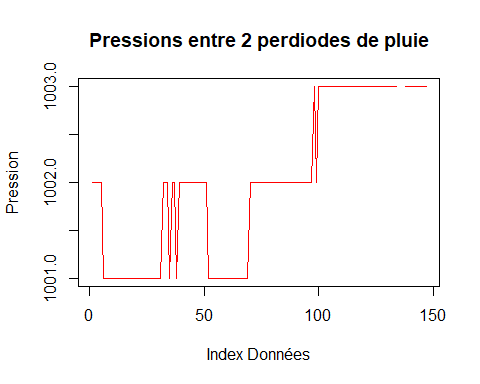
\includegraphics{Rapport_Projet_Data_files/figure-latex/pressure-6.pdf}
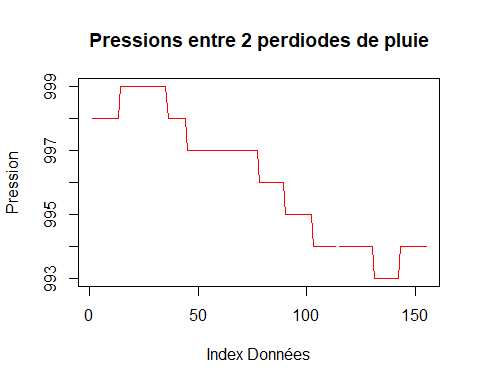
\includegraphics{Rapport_Projet_Data_files/figure-latex/pressure-7.pdf}
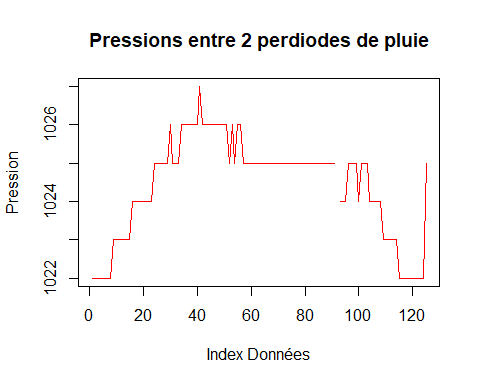
\includegraphics{Rapport_Projet_Data_files/figure-latex/pressure-8.pdf}
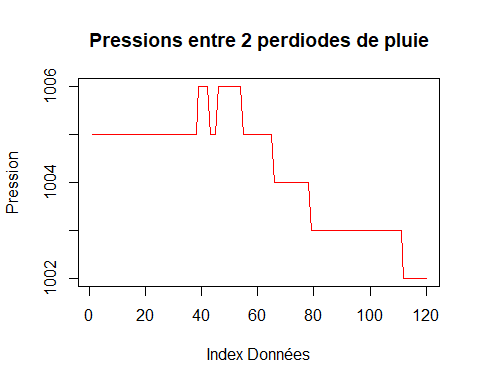
\includegraphics{Rapport_Projet_Data_files/figure-latex/pressure-9.pdf}
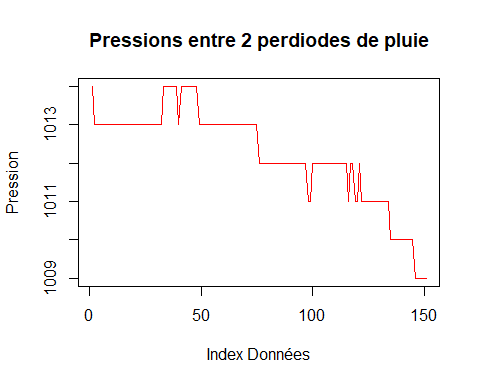
\includegraphics{Rapport_Projet_Data_files/figure-latex/pressure-10.pdf}

Dans l'objective nous voudrions voir une augmentation ou une diminution
de clair de la pression pouvant nous permettre de prédire la pluie sans
trop de risuqe de ce tromper. Ces graphiques montre bien la très faible
corrélation trouvé ci dessus.

\hypertarget{analyse-de-la-tempuxe9rature}{%
\section{Analyse de la température
:}\label{analyse-de-la-tempuxe9rature}}

Toujour dans le même objectif de trouver une variable présentant une
forte corrélation avec la varibale pluie, nous décidons maintenant
d'observer la corelation entre la température et la pluie.

Pour limiter les variation de température lié au cycle jour / nuit du
soleil nous décidons de traiter des données effectué entre 7:00 heure et
21:00 heures.

\begin{Shaded}
\begin{Highlighting}[]
\FunctionTok{cor.test}\NormalTok{(data\_meteo\_jour}\SpecialCharTok{$}\NormalTok{temperature , data\_meteo\_jour}\SpecialCharTok{$}\NormalTok{rain)}
\end{Highlighting}
\end{Shaded}

\begin{verbatim}
## 
##  Pearson's product-moment correlation
## 
## data:  data_meteo_jour$temperature and data_meteo_jour$rain
## t = -51.184, df = 38867, p-value < 2.2e-16
## alternative hypothesis: true correlation is not equal to 0
## 95 percent confidence interval:
##  -0.2605810 -0.2419536
## sample estimates:
##        cor 
## -0.2512906
\end{verbatim}

on observe une corrélation négative relativement forte entre la
temperature et la présense de pluie , ce qui semble logique , la pluis
diminue forcément la température extérieure .

Essayons de regarder maintenant si l'arrivé de la pluie est précédé par
une diminution de la température .

\begin{Shaded}
\begin{Highlighting}[]
\CommentTok{\# }
\CommentTok{\# for (elem in newCollection)\{}
\CommentTok{\#    }
\CommentTok{\# }
\CommentTok{\#     plot( elem[" temperature"], main="temperature  entre 2 perdiodes de pluie",}
\CommentTok{\#           ylab="Temperature ( en degré ° )",}
\CommentTok{\#           xlab="Index Données",}
\CommentTok{\#           type="l",}
\CommentTok{\#           col="blue"  )}
\CommentTok{\# }
\CommentTok{\#   }
\CommentTok{\# \}}
\end{Highlighting}
\end{Shaded}

La température semble effectivement etre assez basse à l'arret de la
pluie et semble dans la plupart des cas léérement diminué lors de
l'arrivée de la pluie mais ces resultats ne semble pas rééllement etre
un moyen de prédire efficassement la pluie .

\hypertarget{analyse-de-lhumidituxe9}{%
\section{Analyse de l'humidité :}\label{analyse-de-lhumidituxe9}}

Nous pensons que l'humidité doit être croissante avant l'arrivé de la
pluie . Nous cherchons tout d'abord à s'avoir si une correlation existe
entre l'humidité et la quantité de Pluie. Toujours limiter les variation
d'humidité lié au cycle jour / nuit du soleil et de la rosée nous
décidons de traiter des données effectué entre 7:00 heure et 21:00
heures.

\begin{Shaded}
\begin{Highlighting}[]
\FunctionTok{cor.test}\NormalTok{(data\_meteo\_jour}\SpecialCharTok{$}\NormalTok{humidity , data\_meteo\_jour}\SpecialCharTok{$}\NormalTok{rain)}\CommentTok{\# 0.30}
\end{Highlighting}
\end{Shaded}

\begin{verbatim}
## 
##  Pearson's product-moment correlation
## 
## data:  data_meteo_jour$humidity and data_meteo_jour$rain
## t = 65.671, df = 41922, p-value < 2.2e-16
## alternative hypothesis: true correlation is not equal to 0
## 95 percent confidence interval:
##  0.2967093 0.3140684
## sample estimates:
##       cor 
## 0.3054142
\end{verbatim}

On observe étonnament une corrélation plus faible que nous ne le
pensions entre la pluie et le pourcentage d'humidité . Nous nous
attendions à trouver un corélation positive et très élévé .

Nous allons donc observer les graphs sur les quelques échantillons
correspondants.

\begin{Shaded}
\begin{Highlighting}[]
\ControlFlowTok{for}\NormalTok{ (elem }\ControlFlowTok{in}\NormalTok{ newCollection)\{}
   

    \FunctionTok{plot}\NormalTok{( elem[}\StringTok{" humidity"}\NormalTok{], }\AttributeTok{main=}\StringTok{"\% Humidité entre 2 perdiodes de pluie"}\NormalTok{,}
          \AttributeTok{ylab=}\StringTok{"humidity ( en degré ° )"}\NormalTok{,}
          \AttributeTok{xlab=}\StringTok{"Index Données"}\NormalTok{,}
          \AttributeTok{type=}\StringTok{"l"}\NormalTok{,}
          \AttributeTok{col=}\StringTok{"blue"}\NormalTok{  )}

  
\NormalTok{\}}
\end{Highlighting}
\end{Shaded}

\includegraphics{Rapport_Projet_Data_files/figure-latex/filter plot temperature echantillons-1.pdf}
\includegraphics{Rapport_Projet_Data_files/figure-latex/filter plot temperature echantillons-2.pdf}
\includegraphics{Rapport_Projet_Data_files/figure-latex/filter plot temperature echantillons-3.pdf}
\includegraphics{Rapport_Projet_Data_files/figure-latex/filter plot temperature echantillons-4.pdf}
\includegraphics{Rapport_Projet_Data_files/figure-latex/filter plot temperature echantillons-5.pdf}
\includegraphics{Rapport_Projet_Data_files/figure-latex/filter plot temperature echantillons-6.pdf}
\includegraphics{Rapport_Projet_Data_files/figure-latex/filter plot temperature echantillons-7.pdf}
\includegraphics{Rapport_Projet_Data_files/figure-latex/filter plot temperature echantillons-8.pdf}
\includegraphics{Rapport_Projet_Data_files/figure-latex/filter plot temperature echantillons-9.pdf}
\includegraphics{Rapport_Projet_Data_files/figure-latex/filter plot temperature echantillons-10.pdf}

On observe que le pourcentage d'humidité est toujours très élevé à la
fin d'une période de pluie par contre l'augmentation de se pourcentage
ne semble pas toujours mené à une pédiode de pluie.

\hypertarget{moyenn-millieu-perdiode-sans-pluie-vs-juste-avant-la-pluie}{%
\subsection{Moyenn millieu perdiode sans pluie vs juste avant la
pluie}\label{moyenn-millieu-perdiode-sans-pluie-vs-juste-avant-la-pluie}}

\begin{Shaded}
\begin{Highlighting}[]
\CommentTok{\# source\_python("C:\textbackslash{}\textbackslash{}Users\textbackslash{}\textbackslash{}sburd\textbackslash{}\textbackslash{}OneDrive\textbackslash{}\textbackslash{}Bureau\textbackslash{}\textbackslash{}Semestre2\textbackslash{}\textbackslash{}Projet\_Data\textbackslash{}\textbackslash{}Stat\textbackslash{}\textbackslash{}Stat\_Projet\_Data\textbackslash{}\textbackslash{}RecupPluieTrue.py")}
\CommentTok{\# monCsv \textless{}{-} openMonCsv("C:\textbackslash{}\textbackslash{}Users\textbackslash{}\textbackslash{}sburd\textbackslash{}\textbackslash{}OneDrive\textbackslash{}\textbackslash{}Bureau\textbackslash{}\textbackslash{}Semestre2\textbackslash{}\textbackslash{}Projet\_Data\textbackslash{}\textbackslash{}DataV2\textbackslash{}\textbackslash{}dataTrainSorti.csv")}
\CommentTok{\# \#heureAdd \textless{}{-} AddHour(monCsv)}
\CommentTok{\# maTabPluie \textless{}{-} trie(monCsv)}
\CommentTok{\# tabDataFrame \textless{}{-} SubsetData(maTabPluie)}
\CommentTok{\# newCollection \textless{}{-} TrieTaille(100,800,tabDataFrame , monCsv)}
\CommentTok{\# TakeDonnePeriode \textless{}{-} MoyenneMidPerdiodeFalsePluieVsBeforePluie(newCollection)}
\CommentTok{\# resMillieu \textless{}{-} resMoyenneMillieu(TakeDonnePeriode[0])}
\CommentTok{\# resBefore \textless{}{-} resMoyenneBefore(TakeDonnePeriode[1])}


\CommentTok{\# \{\textquotesingle{}HumidityM\textquotesingle{}: 47.888888888888886, \textquotesingle{}TemperatureM\textquotesingle{}: 23.9, \textquotesingle{}PressureM\textquotesingle{}: 1004.0, \textquotesingle{}LightM\textquotesingle{}: 529.6666666666666\}}
\CommentTok{\# \{\textquotesingle{}HumidityB\textquotesingle{}: 59.2, \textquotesingle{}TemperatureB\textquotesingle{}: 22.3, \textquotesingle{}PressureB\textquotesingle{}: 1001.4, \textquotesingle{}LightB\textquotesingle{}: 153.6\}}

\CommentTok{\# vM \textless{}{-} c(round(47.888888888888886,2), round(23.9,2), round(1004.0,2), round(529.6666666666666,2))}
\CommentTok{\# valeurMoyenneMillieu\textless{}{-}as.matrix(vM)}
\CommentTok{\# }
\CommentTok{\# vB \textless{}{-} c(round(59.2,1), round(22.3,1), round(1001.4,1), round(153.6,1))}
\CommentTok{\# valeurMoyenneBefore\textless{}{-}as.matrix(vB)}
\CommentTok{\# }
\CommentTok{\# }
\CommentTok{\# barplotvM \textless{}{-} barplot(vM,}
\CommentTok{\#                        col = c("blue", "green", "yellow", "red"),}
\CommentTok{\#                        legend.text = c(paste("Humidité : \% moy : " , round(59.2,2)) ,}
\CommentTok{\#                                        paste("Temperature : température moy : " , round(22.3,2) ,"°C"),}
\CommentTok{\#                                        paste("Pression :  pressions moy" , round(1001.4,2)),}
\CommentTok{\#                                        paste("Lumière :  moy : " , round(153.6,2)) }
\CommentTok{\#                                        ),}
\CommentTok{\#                        main = paste("Graphique montrant la moyenne des \textbackslash{}n variables détécté lors de période de beau temps"),}
\CommentTok{\#                        ylim = c(0,1010),}
\CommentTok{\#                        xlab = "Varaible mesurées",}
\CommentTok{\#                        ylab = "moyenne"}
\CommentTok{\#                        }
\CommentTok{\# )}
\CommentTok{\# }
\CommentTok{\# }
\CommentTok{\# barplotvB \textless{}{-} barplot(vB,}
\CommentTok{\#                        col = c("blue", "green", "yellow", "red"),}
\CommentTok{\#                        legend.text = c(paste("Humidité : \% moy : " , round(47.888888888888886,2)) ,}
\CommentTok{\#                                        paste("Temperature : température moy : " , round(23.9,2) ,"°C"),}
\CommentTok{\#                                        paste("Pression :  pressions moy" , round(1004.0,2)),}
\CommentTok{\#                                        paste("Lumière :  moy : " , round(529.6666666666666,2)) }
\CommentTok{\#                                        ),}
\CommentTok{\#                        main = paste("Graphique montrant la moyenne des \textbackslash{}n variables détécté quelque seconde avant un épisode de pluie"),}
\CommentTok{\#                        ylim = c(0,1010),}
\CommentTok{\#                        xlab = "Varaible mesurées",}
\CommentTok{\#                        ylab = "moyenne"}
\CommentTok{\#                        }
\CommentTok{\# )}


\NormalTok{barplotvM }\OtherTok{\textless{}{-}} \FunctionTok{barplot}\NormalTok{(}\FunctionTok{c}\NormalTok{(}\FunctionTok{round}\NormalTok{(}\FloatTok{47.888888888888886}\NormalTok{,}\DecValTok{2}\NormalTok{) , }\FunctionTok{round}\NormalTok{(}\FloatTok{59.2}\NormalTok{,}\DecValTok{2}\NormalTok{)),}
                       \AttributeTok{col =} \FunctionTok{c}\NormalTok{(}\StringTok{"blue"}\NormalTok{, }\StringTok{"blue"}\NormalTok{),}
                       \AttributeTok{legend.text =} \FunctionTok{c}\NormalTok{(}\FunctionTok{paste}\NormalTok{(}\StringTok{"Humidité perdiode Beau temp: \% moy : "}\NormalTok{ ,}\FunctionTok{round}\NormalTok{(}\FloatTok{47.888888888888886}\NormalTok{,}\DecValTok{2}\NormalTok{) ) ,}
                                       \FunctionTok{paste}\NormalTok{(}\StringTok{"Humidité perdiode avant pluie  : \% moy : "}\NormalTok{ , }\FunctionTok{round}\NormalTok{(}\FloatTok{59.2}\NormalTok{,}\DecValTok{2}\NormalTok{))),}
                       \AttributeTok{main =} \FunctionTok{paste}\NormalTok{(}\StringTok{"Graphique montrant la moyenne des }\SpecialCharTok{\textbackslash{}n}\StringTok{ de l\textquotesingle{}humidité détécté lors de période de beau temps vs perdiode de pré pluie"}\NormalTok{),}
                       \AttributeTok{ylim =} \FunctionTok{c}\NormalTok{(}\DecValTok{0}\NormalTok{,}\DecValTok{100}\NormalTok{),}
                       \AttributeTok{xlab =} \StringTok{"Humidité mesuré"}\NormalTok{,}
                       \AttributeTok{ylab =} \StringTok{"moyenne"}
\NormalTok{)}
\end{Highlighting}
\end{Shaded}

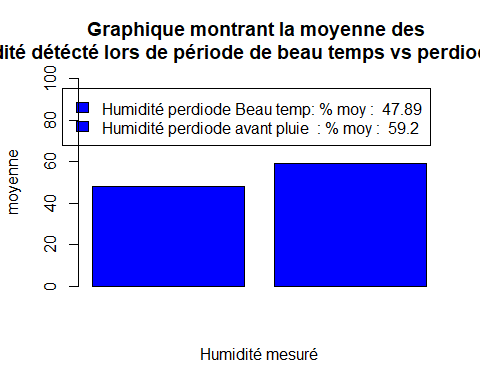
\includegraphics{Rapport_Projet_Data_files/figure-latex/unnamed-chunk-1-1.pdf}

\begin{Shaded}
\begin{Highlighting}[]
\NormalTok{barplotvM }\OtherTok{\textless{}{-}} \FunctionTok{barplot}\NormalTok{(}\FunctionTok{c}\NormalTok{(}\FloatTok{23.9}\NormalTok{ , }\FloatTok{22.3}\NormalTok{),}
                       \AttributeTok{col =} \FunctionTok{c}\NormalTok{(}\StringTok{"red"}\NormalTok{, }\StringTok{"red"}\NormalTok{),}
                       \AttributeTok{legend.text =} \FunctionTok{c}\NormalTok{(}\FunctionTok{paste}\NormalTok{(}\StringTok{"température perdiode Beau temp:  moy : "}\NormalTok{ , }\FloatTok{23.9}\NormalTok{ ) ,}
                                       \FunctionTok{paste}\NormalTok{(}\StringTok{"Humidité perdiode avant pluie  :  moy : "}\NormalTok{ , }\FloatTok{22.3}\NormalTok{)),}
                       \AttributeTok{main =} \FunctionTok{paste}\NormalTok{(}\StringTok{"Graphique montrant la moyenne des }\SpecialCharTok{\textbackslash{}n}\StringTok{ de la temperature détécté lors de période de beau temps vs perdiode de pré pluie"}\NormalTok{),}
                       \AttributeTok{ylim =} \FunctionTok{c}\NormalTok{(}\DecValTok{15}\NormalTok{,}\DecValTok{28}\NormalTok{),}
                       \AttributeTok{xlab =} \StringTok{"temperature mesuré"}\NormalTok{,}
                       \AttributeTok{ylab =} \StringTok{"moyenne"}
\NormalTok{)}
\end{Highlighting}
\end{Shaded}

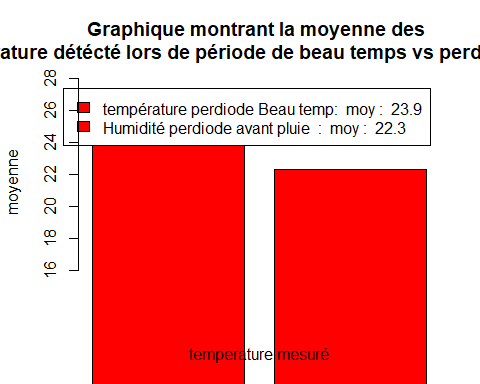
\includegraphics{Rapport_Projet_Data_files/figure-latex/unnamed-chunk-1-2.pdf}

\begin{Shaded}
\begin{Highlighting}[]
\NormalTok{barplotvM }\OtherTok{\textless{}{-}} \FunctionTok{barplot}\NormalTok{(}\FunctionTok{c}\NormalTok{(}\FloatTok{1004.0}\NormalTok{ , }\FloatTok{1001.2}\NormalTok{),}
                       \AttributeTok{col =} \FunctionTok{c}\NormalTok{(}\StringTok{"green"}\NormalTok{, }\StringTok{"green"}\NormalTok{),}
                       \AttributeTok{legend.text =} \FunctionTok{c}\NormalTok{(}\FunctionTok{paste}\NormalTok{(}\StringTok{"Pression perdiode Beau temp:  moy : "}\NormalTok{ , }\FloatTok{1004.0}\NormalTok{ ) ,}
                                       \FunctionTok{paste}\NormalTok{(}\StringTok{"Pression perdiode avant pluie  :  moy : "}\NormalTok{ , }\FloatTok{1001.2}\NormalTok{)),}
                       \AttributeTok{main =} \FunctionTok{paste}\NormalTok{(}\StringTok{"Graphique montrant la moyenne des }\SpecialCharTok{\textbackslash{}n}\StringTok{ de la Pression détécté lors de période de beau temps vs perdiode de pré pluie"}\NormalTok{),}
                       \AttributeTok{ylim =} \FunctionTok{c}\NormalTok{(}\DecValTok{998}\NormalTok{,}\DecValTok{1005}\NormalTok{),}
                       \AttributeTok{xlab =} \StringTok{"Pression mesuré"}\NormalTok{,}
                       \AttributeTok{ylab =} \StringTok{"moyenne"}
\NormalTok{)}
\end{Highlighting}
\end{Shaded}

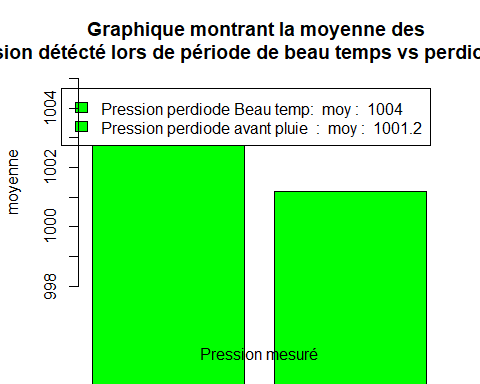
\includegraphics{Rapport_Projet_Data_files/figure-latex/unnamed-chunk-1-3.pdf}

\begin{Shaded}
\begin{Highlighting}[]
\NormalTok{barplotvM }\OtherTok{\textless{}{-}} \FunctionTok{barplot}\NormalTok{(}\FunctionTok{c}\NormalTok{(}\FloatTok{529.6666666666666}\NormalTok{ , }\FloatTok{153.6}\NormalTok{),}
                       \AttributeTok{col =} \FunctionTok{c}\NormalTok{(}\StringTok{"yellow"}\NormalTok{, }\StringTok{"yellow"}\NormalTok{),}
                       \AttributeTok{legend.text =} \FunctionTok{c}\NormalTok{(}\FunctionTok{paste}\NormalTok{(}\StringTok{"Lumière perdiode Beau temp:  moy : "}\NormalTok{ , }\FloatTok{529.66}\NormalTok{ ) ,}
                                       \FunctionTok{paste}\NormalTok{(}\StringTok{"Lumière perdiode avant pluie  :  moy : "}\NormalTok{ , }\FloatTok{153.6}\NormalTok{)),}
                       \AttributeTok{main =} \FunctionTok{paste}\NormalTok{(}\StringTok{"Graphique montrant la moyenne des }\SpecialCharTok{\textbackslash{}n}\StringTok{ de la Lumière détécté lors de période de beau temps vs perdiode de pré pluie"}\NormalTok{),}
                       \AttributeTok{ylim =} \FunctionTok{c}\NormalTok{(}\DecValTok{120}\NormalTok{,}\DecValTok{560}\NormalTok{),}
                       \AttributeTok{xlab =} \StringTok{"Lumière mesuré"}\NormalTok{,}
                       \AttributeTok{ylab =} \StringTok{"moyenne"}
\NormalTok{)}
\end{Highlighting}
\end{Shaded}

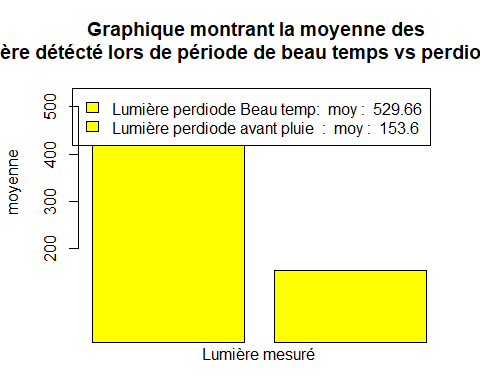
\includegraphics{Rapport_Projet_Data_files/figure-latex/unnamed-chunk-1-4.pdf}

On observe que la moyenne d'humidité juste avant une période de pluie
est plus élévé de presque 10 point . La température moyenne perd presque
1 degré juste avant une période de pluie . La pression atmosphérique
moyenne est au alentour de 1001 juste avant une période de pluie alors
qu'elle est au alentour de 1004 lors de période de beau temps . La
lumière détécté est quand à elle presque 4 fois supérieure lors de
période de beau temps . c'est information semble montrer qu'une période
de pluie peut finalement etre prédit lorsque l'on regarde les moyennes .

\hypertarget{facteur-dhumidituxe9-en-hiver}{%
\subsection{Facteur d'humidité en
hiver}\label{facteur-dhumidituxe9-en-hiver}}

Nous émetons l'hipothèse que le facteur d'humidité est un facteur
annonciateur de la pluie plus conséquent en hiver que pendant les autres
saisons.

\begin{Shaded}
\begin{Highlighting}[]
\NormalTok{data\_meteo\_season}\SpecialCharTok{$}\NormalTok{month }\OtherTok{\textless{}{-}} \FunctionTok{strtoi}\NormalTok{(}\FunctionTok{str\_sub}\NormalTok{(data\_meteo}\SpecialCharTok{$}\NormalTok{date..date, }\DecValTok{7}\NormalTok{, }\DecValTok{8}\NormalTok{))}

\NormalTok{data\_meteo\_season}\SpecialCharTok{$}\NormalTok{season}\OtherTok{\textless{}{-}}\StringTok{"summer"}
\NormalTok{data\_meteo\_season}\SpecialCharTok{$}\NormalTok{season[data\_meteo\_season}\SpecialCharTok{$}\NormalTok{month}\SpecialCharTok{\textgreater{}}\DecValTok{9}\SpecialCharTok{\&}\NormalTok{data\_meteo\_season}\SpecialCharTok{$}\NormalTok{month}\SpecialCharTok{\textless{}=}\DecValTok{12}\NormalTok{]}\OtherTok{\textless{}{-}}\StringTok{"autumn"}
\NormalTok{data\_meteo\_season}\SpecialCharTok{$}\NormalTok{season[data\_meteo\_season}\SpecialCharTok{$}\NormalTok{month}\SpecialCharTok{\textgreater{}}\DecValTok{1}\SpecialCharTok{\&}\NormalTok{data\_meteo\_season}\SpecialCharTok{$}\NormalTok{month}\SpecialCharTok{\textless{}=}\DecValTok{3}\NormalTok{]}\OtherTok{\textless{}{-}}\StringTok{"winter"}
\NormalTok{data\_meteo\_season}\SpecialCharTok{$}\NormalTok{season[data\_meteo\_season}\SpecialCharTok{$}\NormalTok{month}\SpecialCharTok{\textgreater{}}\DecValTok{3}\SpecialCharTok{\&}\NormalTok{data\_meteo\_season}\SpecialCharTok{$}\NormalTok{month}\SpecialCharTok{\textless{}=}\DecValTok{6}\NormalTok{]}\OtherTok{\textless{}{-}}\StringTok{"spring"}
\NormalTok{data\_meteo\_season}\SpecialCharTok{$}\NormalTok{season}\OtherTok{\textless{}{-}}\FunctionTok{factor}\NormalTok{(data\_meteo\_season}\SpecialCharTok{$}\NormalTok{season,}\AttributeTok{levels=}\FunctionTok{c}\NormalTok{(}\StringTok{"summer"}\NormalTok{,}\StringTok{"spring"}\NormalTok{,}\StringTok{"winter"}\NormalTok{,}\StringTok{"autumn"}\NormalTok{))}


\NormalTok{summer }\OtherTok{\textless{}{-}} \FunctionTok{filter}\NormalTok{(data\_meteo\_season, season }\SpecialCharTok{==} \StringTok{"summer"}\NormalTok{, rain }\SpecialCharTok{!=} \StringTok{"NA"}\NormalTok{, humidity }\SpecialCharTok{!=} \StringTok{"NA"}\NormalTok{, temperature }\SpecialCharTok{!=} \StringTok{"NA"}\NormalTok{)}
\NormalTok{autumn }\OtherTok{\textless{}{-}} \FunctionTok{filter}\NormalTok{(data\_meteo\_season, season }\SpecialCharTok{==} \StringTok{"autumn"}\NormalTok{, rain }\SpecialCharTok{!=} \StringTok{"NA"}\NormalTok{, humidity }\SpecialCharTok{!=} \StringTok{"NA"}\NormalTok{,  temperature }\SpecialCharTok{!=} \StringTok{"NA"}\NormalTok{)}
\NormalTok{spring }\OtherTok{\textless{}{-}} \FunctionTok{filter}\NormalTok{(data\_meteo\_season, season }\SpecialCharTok{==} \StringTok{"spring"}\NormalTok{, rain }\SpecialCharTok{!=} \StringTok{"NA"}\NormalTok{, humidity }\SpecialCharTok{!=} \StringTok{"NA"}\NormalTok{,  temperature }\SpecialCharTok{!=} \StringTok{"NA"}\NormalTok{)}
\NormalTok{winter }\OtherTok{\textless{}{-}} \FunctionTok{filter}\NormalTok{(data\_meteo\_season, season }\SpecialCharTok{==} \StringTok{"winter"}\NormalTok{, rain }\SpecialCharTok{!=} \StringTok{"NA"}\NormalTok{, humidity }\SpecialCharTok{!=} \StringTok{"NA"}\NormalTok{,  temperature }\SpecialCharTok{!=} \StringTok{"NA"}\NormalTok{)}

\NormalTok{corWin }\OtherTok{=} \FunctionTok{cor}\NormalTok{( winter}\SpecialCharTok{$}\NormalTok{humidity, winter}\SpecialCharTok{$}\NormalTok{rain, }\AttributeTok{method=}\FunctionTok{c}\NormalTok{(}\StringTok{"pearson"}\NormalTok{, }\StringTok{"kendall"}\NormalTok{, }\StringTok{"spearman"}\NormalTok{)) }\CommentTok{\#0.4774225}
\NormalTok{corSum }\OtherTok{=} \FunctionTok{cor}\NormalTok{( summer}\SpecialCharTok{$}\NormalTok{humidity, summer}\SpecialCharTok{$}\NormalTok{rain, }\AttributeTok{method=}\FunctionTok{c}\NormalTok{(}\StringTok{"pearson"}\NormalTok{, }\StringTok{"kendall"}\NormalTok{, }\StringTok{"spearman"}\NormalTok{)) }\CommentTok{\#0.2675425}
\NormalTok{corAut }\OtherTok{=} \FunctionTok{cor}\NormalTok{( autumn}\SpecialCharTok{$}\NormalTok{humidity, autumn}\SpecialCharTok{$}\NormalTok{rain, }\AttributeTok{method=}\FunctionTok{c}\NormalTok{(}\StringTok{"pearson"}\NormalTok{, }\StringTok{"kendall"}\NormalTok{, }\StringTok{"spearman"}\NormalTok{)) }\CommentTok{\#0.313826}
\NormalTok{corSpr }\OtherTok{=} \FunctionTok{cor}\NormalTok{( spring}\SpecialCharTok{$}\NormalTok{humidity, spring}\SpecialCharTok{$}\NormalTok{rain, }\AttributeTok{method=}\FunctionTok{c}\NormalTok{(}\StringTok{"pearson"}\NormalTok{, }\StringTok{"kendall"}\NormalTok{, }\StringTok{"spearman"}\NormalTok{)) }\CommentTok{\#  0.3957939}




\NormalTok{CorSaisVal}\OtherTok{\textless{}{-}}\FunctionTok{as.matrix}\NormalTok{(}\FunctionTok{c}\NormalTok{(corWin, corSpr, corSum, corAut))}



\NormalTok{barplotsais }\OtherTok{\textless{}{-}} \FunctionTok{barplot}\NormalTok{(}\FunctionTok{c}\NormalTok{(corWin, corSpr, corSum, corAut),}
                       \AttributeTok{col =} \FunctionTok{c}\NormalTok{(}\StringTok{"blue"}\NormalTok{, }\StringTok{"green"}\NormalTok{, }\StringTok{"yellow"}\NormalTok{, }\StringTok{"red"}\NormalTok{),}
                       \AttributeTok{legend.text =} \FunctionTok{c}\NormalTok{(}\FunctionTok{paste}\NormalTok{(}\StringTok{"Hiver : température moy : "}\NormalTok{ , }\FunctionTok{round}\NormalTok{(}\FunctionTok{mean}\NormalTok{(winter}\SpecialCharTok{$}\NormalTok{temperature), }\DecValTok{1}\NormalTok{),}\StringTok{"°C"}\NormalTok{) ,}
                                       \FunctionTok{paste}\NormalTok{(}\StringTok{"Printemps : température moy : "}\NormalTok{ , }\FunctionTok{round}\NormalTok{(}\FunctionTok{mean}\NormalTok{(spring}\SpecialCharTok{$}\NormalTok{temperature), }\DecValTok{1}\NormalTok{),}\StringTok{"°C"}\NormalTok{),}
                                       \FunctionTok{paste}\NormalTok{(}\StringTok{"été :  température moy"}\NormalTok{ , }\FunctionTok{round}\NormalTok{(}\FunctionTok{mean}\NormalTok{(summer}\SpecialCharTok{$}\NormalTok{temperature), }\DecValTok{1}\NormalTok{),}\StringTok{"°C"}\NormalTok{),}
                                       \FunctionTok{paste}\NormalTok{(}\StringTok{"Automne : température moy : "}\NormalTok{ , }\FunctionTok{round}\NormalTok{(}\FunctionTok{mean}\NormalTok{(autumn}\SpecialCharTok{$}\NormalTok{temperature), }\DecValTok{1}\NormalTok{),}\StringTok{"°C"}\NormalTok{) }
\NormalTok{                                       ),}
                       \AttributeTok{main =} \FunctionTok{paste}\NormalTok{(}\StringTok{"Graphique montrant la corrélation entre }\SpecialCharTok{\textbackslash{}n}\StringTok{ l\textquotesingle{}humidité et la pluie selon la saison"}\NormalTok{),}
                       \AttributeTok{ylim =} \FunctionTok{c}\NormalTok{(}\DecValTok{0}\NormalTok{,}\FloatTok{0.5}\NormalTok{),}
                       \AttributeTok{xlab =} \StringTok{"Saison"}\NormalTok{,}
                       \AttributeTok{ylab =} \StringTok{"Corrélation"}
                       
\NormalTok{)}

\FunctionTok{text}\NormalTok{(barplotsais ,CorSaisVal}\FloatTok{+0.02}\NormalTok{,}\AttributeTok{labels=}\FunctionTok{round}\NormalTok{(CorSaisVal,}\DecValTok{2}\NormalTok{)) }
\end{Highlighting}
\end{Shaded}

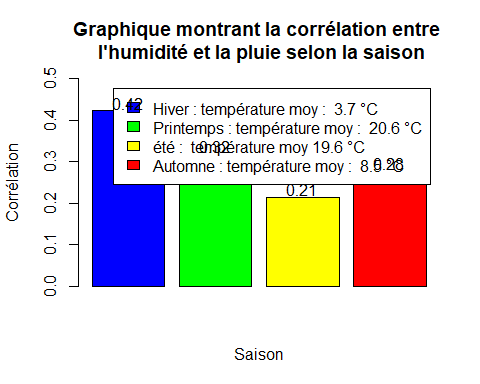
\includegraphics{Rapport_Projet_Data_files/figure-latex/saison-1.pdf}
D'après les données recueillit, nous pouvons constater que plus la
saison est froide, plus le taux d'humidité est en corrélation avec
l'arrivé de la pluie.

L'hypothèse suggèrant que le facteur d'humidité est un facteur plus
conséquent selon la saison est validée, sur le graphique ci-dessus, nous
constatons que la corrélation entre l'humidité et la pluie est prêts de
deux fois supérieur en hiver que pendant une autre saison.

À partir de ces résultats, nous pourrons donner plus d'importances à la
valeur d'humidité selon la saison et selon la température.

\hypertarget{le-cycle-journuit-jour-sur-la-pluie}{%
\subsection{Le cycle jour/nuit jour sur la
pluie}\label{le-cycle-journuit-jour-sur-la-pluie}}

Nous émétons l'hypothèse que la nuit est un facteur annonciateur de la
pluie.

\begin{Shaded}
\begin{Highlighting}[]
\NormalTok{data\_meteo\_rain }\OtherTok{\textless{}{-}}\NormalTok{ data\_meteo}
\NormalTok{data\_meteo\_rain }\OtherTok{\textless{}{-}} \FunctionTok{filter}\NormalTok{(data\_meteo\_rain, rain }\SpecialCharTok{!=} \StringTok{"NA"} \SpecialCharTok{\&}\NormalTok{ light }\SpecialCharTok{!=} \StringTok{"NA"}\NormalTok{)}

\NormalTok{data\_meteo\_rain}\SpecialCharTok{$}\NormalTok{pluie[data\_meteo\_rain}\SpecialCharTok{$}\NormalTok{rain}\SpecialCharTok{\textgreater{}}\DecValTok{0}\NormalTok{]}\OtherTok{\textless{}{-}}\StringTok{"oui"}
\NormalTok{data\_meteo\_rain}\SpecialCharTok{$}\NormalTok{pluie[data\_meteo\_rain}\SpecialCharTok{$}\NormalTok{rain}\SpecialCharTok{==}\DecValTok{0}\NormalTok{]}\OtherTok{\textless{}{-}}\StringTok{"non"}
\NormalTok{data\_meteo\_rain}\SpecialCharTok{$}\NormalTok{jour[data\_meteo\_rain}\SpecialCharTok{$}\NormalTok{light}\SpecialCharTok{\textgreater{}}\DecValTok{0}\NormalTok{]}\OtherTok{\textless{}{-}}\StringTok{"jour"}
\NormalTok{data\_meteo\_rain}\SpecialCharTok{$}\NormalTok{jour[data\_meteo\_rain}\SpecialCharTok{$}\NormalTok{light}\SpecialCharTok{==}\DecValTok{0}\NormalTok{]}\OtherTok{\textless{}{-}}\StringTok{"nuit"}

\NormalTok{data\_meteo\_jour }\OtherTok{\textless{}{-}} \FunctionTok{filter}\NormalTok{(data\_meteo\_rain, jour }\SpecialCharTok{==} \StringTok{"jour"}\NormalTok{)}
\NormalTok{data\_meteo\_nuit }\OtherTok{\textless{}{-}} \FunctionTok{filter}\NormalTok{(data\_meteo\_rain, jour }\SpecialCharTok{==} \StringTok{"nuit"}\NormalTok{)}

\NormalTok{effectifsjour }\OtherTok{\textless{}{-}} \FunctionTok{table}\NormalTok{(data\_meteo\_jour}\SpecialCharTok{$}\NormalTok{pluie)}
\NormalTok{racajour}\OtherTok{=}\FunctionTok{prop.table}\NormalTok{(effectifsjour) }\SpecialCharTok{*} \DecValTok{100}
\NormalTok{effectifsnuit }\OtherTok{\textless{}{-}} \FunctionTok{table}\NormalTok{(data\_meteo\_nuit}\SpecialCharTok{$}\NormalTok{pluie)}
\NormalTok{racanuit}\OtherTok{=}\FunctionTok{prop.table}\NormalTok{(effectifsnuit) }\SpecialCharTok{*} \DecValTok{100}

\NormalTok{pcrjp7}\OtherTok{\textless{}{-}}\FunctionTok{as.matrix}\NormalTok{(}\FunctionTok{c}\NormalTok{(racajour[}\StringTok{"oui"}\NormalTok{],  racanuit[}\StringTok{"oui"}\NormalTok{]))}
\NormalTok{pcrjp}\OtherTok{\textless{}{-}}\FunctionTok{as.matrix}\NormalTok{(}\FunctionTok{c}\NormalTok{(pcrjp7[}\DecValTok{1}\NormalTok{], pcrjp7[}\DecValTok{2}\NormalTok{]))}


\NormalTok{barplotjp }\OtherTok{=} \FunctionTok{barplot}\NormalTok{(}\FunctionTok{table}\NormalTok{(data\_meteo\_rain}\SpecialCharTok{$}\NormalTok{pluie, data\_meteo\_rain}\SpecialCharTok{$}\NormalTok{jour),}
        \AttributeTok{col =} \FunctionTok{c}\NormalTok{(}\StringTok{"yellow"}\NormalTok{, }\StringTok{"blue"}\NormalTok{),}
        \AttributeTok{legend.text =} \FunctionTok{c}\NormalTok{(}\FunctionTok{paste}\NormalTok{(}\StringTok{"Pas de pluie "}\NormalTok{) ,}
                        \FunctionTok{paste}\NormalTok{(}\StringTok{"pluie "}\NormalTok{)}
\NormalTok{        ),}
        \AttributeTok{main =} \FunctionTok{paste}\NormalTok{(}\StringTok{"Graphique montrant le pourcentage de pluie }\SpecialCharTok{\textbackslash{}n}\StringTok{ selon la journée ou la nuit."}\NormalTok{),}
        \AttributeTok{ylim =} \FunctionTok{c}\NormalTok{(}\DecValTok{0}\NormalTok{,}\DecValTok{60000}\NormalTok{),}
        \AttributeTok{xlab =} \StringTok{"periode"}\NormalTok{,}
        \AttributeTok{ylab =} \StringTok{"détéction de pluie"}
\NormalTok{        )}

\FunctionTok{text}\NormalTok{(barplotjp ,pcrjp}\SpecialCharTok{+}\DecValTok{45000}\NormalTok{,}\AttributeTok{labels=}\FunctionTok{as.character}\NormalTok{(}\FunctionTok{paste}\NormalTok{(}\FunctionTok{round}\NormalTok{(pcrjp,}\DecValTok{1}\NormalTok{),}\StringTok{"\%"}\NormalTok{))) }
\end{Highlighting}
\end{Shaded}

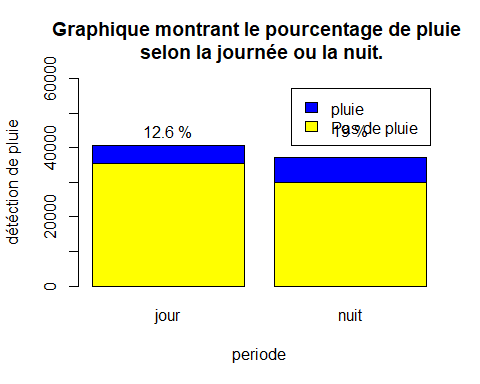
\includegraphics{Rapport_Projet_Data_files/figure-latex/jour/nuit + pluie-1.pdf}

D'après les données recueillit, non pouvons constater sur le graphique
précédant qu'il n'y pas de différence significative entre le jour et la
nuit.

L'hypothèse signifiant que le le jour ou la nuit sont des facteurs plus
conséquents, est donc fausse malgré le fait que nous avons une petite
augmentation de pluie la nuit.

D'après ces résultats, nous savons que le cycle jour nuit n'est pas un
facteur assez déterminant pour le prendre en compte lors de la mise en
place de l'algorithme de détection de pluie.

\end{document}
